\section{Extension Results} \label{sec:extension-results}

Figure \ref{fig:extension_plot} shows the results produced by the EXGA\_1 and EXGA\_2 algorithms plotted on top of the reimplemented figure. 

It can be seen that the EXGA\_1 and EXGA\_2 algorithms do indeed perform slightly better on the Rastrigin and Schwefel functions, with EXGA\_2 performing slightly better than EXGA\_1 in both cases.
However, they perform worse that the standard GA on the Griewangk and Ackley Functions.

It is thought this difference in performance comes from the interdependency between parameters in the Griewangk and Ackley functions. 
These functions have a higher epistasis than the Rastrigin or Schwefel functions and using two point crossover preserves more of the genetic background along with any good genes developed.

The CCGA maintains a relative performance increase over all other tested algorithms as each gene is evaluated in the context of the other best performing genes. 
The performance of each new gene is measured in this context so sudden shifts in the genetic background are less likely than in EXGA\_1 and EXGA\_2.

\begin{figure}[ht!]
    \centering 
    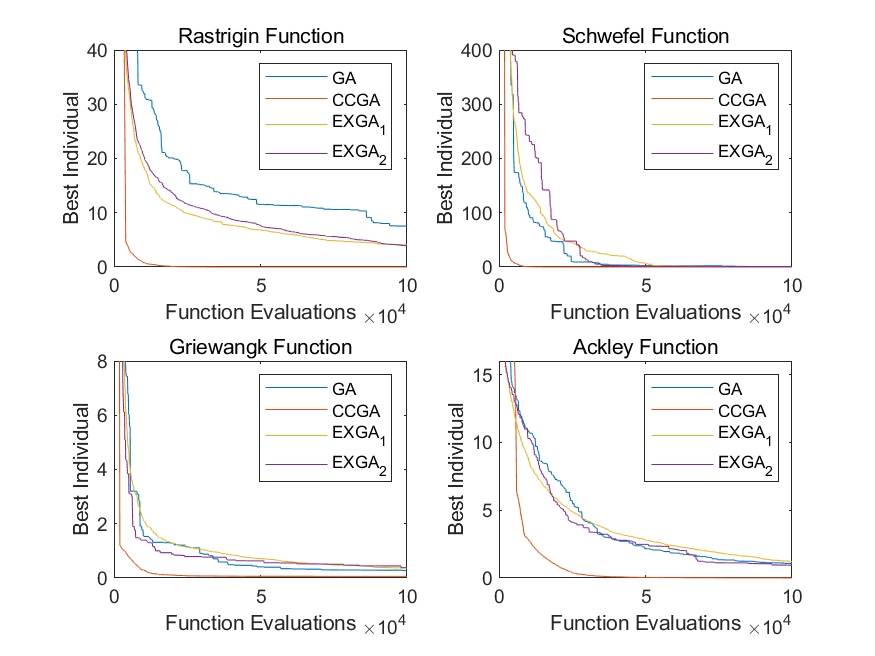
\includegraphics[width=0.9\textwidth]{img/extension_plot.png}
    \caption{The figure produced to demonstrate the extension produced for this assignment.}
    \label{fig:extension_plot}
  \end{figure}
